\chapter{Specifikacija programske potpore}
		
	\section{Funkcionalni zahtjevi}
			
			\textbf{\textit{dio 1. revizije}}\\
			
			\noindent \textbf{Dionici:}
			
			\begin{packed_enum}
				\item Gradska uprava
				\item Djelatnici gradskih ureda		
				\item Građani grada
				\item[] \begin{packed_item}
					\item Registrirani korisnici
					\item Neregistrirani korisnici
				\end{packed_item}
				\item Razvojni tim
			\end{packed_enum}
			
			
			\noindent \textbf{Aktori i njihovi funkcionalni zahtjevi:}
			
			\begin{packed_enum}
				
				\item  \underbar{Neregistrirani korisnik (inicijator) može:}
				\begin{packed_enum}
					\item napraviti svoj profil za koji mu je potrebno ime, prezime, datum rođenja, email adresa, lozinka i opcionalno profilna slika
					\item podnositi anonimnu prijavu koja sadrži naslov, opis, lokaciju i nadležni gradski ured, a opcionalno i fotografiju i prijavu na koju se nadovezuje
					\item  pregledavati postojeće prijave preko liste ili karte te ih filtrirati po lokaciji, vremenu, statusu i nadležnom gradskom uredu
					\item pregledavati statistiku postojećih prijava za odabran period, lokaciju i nadležan gradski ured			
				\end{packed_enum}
								
				\item  \underbar{Registrirani korisnik (inicijator) može:}				
				\begin{packed_enum}					
					\item pregledavati i mijenjati osobne podatke
					\item obrisati svoj profil
					\item pregledavati svoje prošle prijave
					\item podnositi prijavu koja sadrži naslov, opis, lokaciju i nadležni gradski ured, a opcionalno i fotografiju i prijavu na koju se nadovezuje
					\item  pregledavati postojeće prijave preko liste ili karte te ih filtrirati po lokaciji, vremenu, statusu i nadležnom gradskom uredu
					\item pregledavati statistiku postojećih prijava za odabran period, lokaciju i nadležan gradski ured
				\end{packed_enum}
				
				\item  \underbar{Djelatnik gradskog ureda (inicijator) može:}
				\begin{packed_enum}
					\item pregledavati prijave pristigle u njihov ured prema njihovom statusu
					\item prijavama sa statusom \textit{na čekanju} mijenjati status u \textit{u procesu rješavanja}
					\item prijavama sa statusom \textit{u procesu rješavanja} mijenjati status u \textit{riješena}
					\item objediniti prijave ako se referiraju na isti problem
					\item pregledavati prijave na karti
					\item pregledavati statistiku prijava pristiglih u njihov ured
				\end{packed_enum}
				
				\item  \underbar{Baza podataka (sudionik) može:}
				\begin{packed_enum}
					\item spremati sve podatke o korisnicima
					\item spremati sve podatke o prijavama
				\end{packed_enum}
				
			\end{packed_enum}
						
			\eject 
			
				
						
			\subsection{Obrasci uporabe}
				
				\textbf{\textit{dio 1. revizije}}

					\noindent \underbar{\textbf{UC1 - Prijava oštećenja}}
					\begin{packed_item}
	
						\item \textbf{Glavni sudionik:} Korisnik
						\item  \textbf{Cilj:} Prijaviti oštećenje nadležnom gradskom uredu
						\item  \textbf{Sudionici:} Gradski ured, Baza podataka
						\item  \textbf{Preduvjet:} Korisnik je pronašao oštećenje koje želi prijaviti
						
						\item  \textbf{Opis osnovnog tijeka:}
						\item[] \begin{packed_enum}
							\item Korisnik odabire opciju za prijavljivanje oštećenja
							\item Korisnik popunjava podatke za prijavu oštećenja i podnosi prijavu
							\item Prijava se sprema u bazu podataka
							\item Korisnik dobiva jedinstveni kod svoje prijave.
						\end{packed_enum}
						
						\item  \textbf{Opis mogućih odstupanja:}
						\item[] \begin{packed_item}
							\item[2.a] Korisnik nije unio sve obavezne podatke u prijavu.
							\item[] \begin{packed_enum}
								\item Korisnik dobiva obavijest.
								\item Korisnik popunjava preostala obavezna polja ili odustaje od podnošenja prijave
							\end{packed_enum}
							
						\end{packed_item}
					\end{packed_item}
					
					
					\noindent \underbar{\textbf{UC2 - Pregled svih prijava}}
					\begin{packed_item}
						
						\item \textbf{Glavni sudionik:} Korisnik
						\item  \textbf{Cilj:} Pregled aktivnih prijava u sustavu
						\item  \textbf{Sudionici:} Baza podataka
						\item  \textbf{Preduvjet:} -
						
						\item  \textbf{Opis osnovnog tijeka:}
						\item[] \begin{packed_enum}
							\item Korisnik odabire opciju za pregledavanje prijava
							\item Aplikacija prikazuje prijave
							\item Korisnik odabire prijavu
							\item Prikazuju se podaci o prijavi
						\end{packed_enum}
					\end{packed_item}
				
				
				\noindent \underbar{\textbf{UC3 - Filtriranje prijava}}
				\begin{packed_item}
					
					\item \textbf{Glavni sudionik:} Korisnik
					\item  \textbf{Cilj:} Filtriranje prijava prilikom pregleda
					\item  \textbf{Sudionici:} Baza podataka
					\item  \textbf{Preduvjet:} Korisnik je odabrao opciju pregleda svih prijava
					
					\item  \textbf{Opis osnovnog tijeka:}
					\item[] \begin{packed_enum}
						\item Korisnik odabire opcije kod filtriranja
						\item Aplikacija prikazuje filtrirane prijave
					\end{packed_enum}
					
					\item  \textbf{Opis mogućih odstupanja:}
					\item[] \begin{packed_item}
						\item[1.a] Korisnik ne želi filtrirati prijave
						\item[] \begin{packed_enum}
							\item Aplikacija prikazuje nefiltrirane prijave
						\end{packed_enum}
						
					\end{packed_item}
				\end{packed_item}
				
				
				\noindent \underbar{\textbf{UC4 - Pregled statistike prijava}}
				\begin{packed_item}
					
					\item \textbf{Glavni sudionik:} Korisnik ili Djelatnik gradskog ureda
					\item  \textbf{Cilj:} Pregled statistike prijava u sustavu
					\item  \textbf{Sudionici:} Baza podataka
					\item  \textbf{Preduvjet:} -
					
					\item  \textbf{Opis osnovnog tijeka:}
					\item[] \begin{packed_enum}
						\item Korisnik odabire opciju za pregledavanje statistike prijava
						\item Aplikacija prikazuje razne podatke za prijave u sustavu
					\end{packed_enum}
				\end{packed_item}
				
				
				\noindent \underbar{\textbf{UC5 - Filtriranje statistike prijava}}
				\begin{packed_item}
					
					\item \textbf{Glavni sudionik:} Korisnik ili Djelatnik Gradskog ureda
					\item  \textbf{Cilj:} Filtriranje prijava prilikom pregleda statistike
					\item  \textbf{Sudionici:} Baza podataka
					\item  \textbf{Preduvjet:} Korisnik je odabrao opciju pregleda statistike prijava
					
					\item  \textbf{Opis osnovnog tijeka:}
					\item[] \begin{packed_enum}
						\item Korisnik odabire opcije za filtriranje
						\item Aplikacija prikazuje statistiku za filtrirane prijave
					\end{packed_enum}
				\end{packed_item}
				
				
				\noindent \underbar{\textbf{UC6 - Registracija}}
				\begin{packed_item}
					
					\item \textbf{Glavni sudionik:} Neregistrirani korisnik ili Djelatnik gradskog ureda
					\item  \textbf{Cilj:} Izrada korisničkog računa za korisnika ili novi gradski ured
					\item  \textbf{Sudionici:} Baza podataka
					\item  \textbf{Preduvjet:} -
					
					\item  \textbf{Opis osnovnog tijeka:}
					\item[] \begin{packed_enum}
						\item Korisnik odabire opciju registracije
						\item Korisnik popunjava podatke za izradu korisničkog računa i potvrđuje registraciju
					\end{packed_enum}
					
					\item  \textbf{Opis mogućih odstupanja:}
					\item[] \begin{packed_item}
						\item[2.a] Unesena email adresa je već zauzeta
						\item[] \begin{packed_enum}
							\item Aplikacija prikazuje prikladnu obavijest i vraća korisnika na stranicu za registraciju
							\item Korisnik unosi drugu email adresu ili odustaje od registracije
						\end{packed_enum}
					\end{packed_item}
				\end{packed_item}
				
				
				\noindent \underbar{\textbf{UC7 - Pregled vlastitih prijava}}
				\begin{packed_item}
					
					\item \textbf{Glavni sudionik:} Registrirani korisnik
					\item  \textbf{Cilj:} Pregled prijava koje je korisnik do sada podnio
					\item  \textbf{Sudionici:} Baza podataka
					\item  \textbf{Preduvjet:} -
					
					\item  \textbf{Opis osnovnog tijeka:}
					\item[] \begin{packed_enum}
						\item Registrirani korisnik odabire ikonu svojeg profila
						\item Registrirani korisnik na ponuđenom izborniku odabire opciju pregleda vlastitih prijava
						\item Aplikacija prikazuje listu dosadašnjih prijava Registriranog korisnika
						\item Registrirani korisnik odabire prijavu
						\item Prikazuju se podaci o prijavi
					\end{packed_enum}
					
					\item  \textbf{Opis mogućih odstupanja:}
					\item[] \begin{packed_item}
						\item[4.a] Registrirani korisnik nema podnesenih prijava
						\item[] \begin{packed_enum}
							\item Aplikacija prikazuje praznu listu
							\item Registrirani korisnik odustaje od pregleda vlastitih prijava
						\end{packed_enum}
					\end{packed_item}
				\end{packed_item}
				
				
				\noindent \underbar{\textbf{UC8 - Pregled podataka o računu}}
				\begin{packed_item}
					
					\item \textbf{Glavni sudionik:} Registrirani korisnik
					\item  \textbf{Cilj:} Pregled podataka o korisničkom računu
					\item  \textbf{Sudionici:} Baza podataka
					\item  \textbf{Preduvjet:} -
					
					\item  \textbf{Opis osnovnog tijeka:}
					\item[] \begin{packed_enum}
						\item Registrirani korisnik odabire ikonu svojeg profila
						\item Registrirani korisnik na ponuđenom izborniku odabire opciju pregleda podataka o računu
						\item Aplikacija prikazuje podatke o korisničkom računu
					\end{packed_enum}
				\end{packed_item}
				
				
				\noindent \underbar{\textbf{UC9 - Promjena podataka o računu}}
				\begin{packed_item}
					
					\item \textbf{Glavni sudionik:} Registrirani korisnik
					\item  \textbf{Cilj:} Promjena podataka o korisničkom računu
					\item  \textbf{Sudionici:} Baza podataka
					\item  \textbf{Preduvjet:} -
					
					\item  \textbf{Opis osnovnog tijeka:}
					\item[] \begin{packed_enum}
						\item Registrirani korisnik odabire ikonu svojeg profila
						\item Registrirani korisnik na ponuđenom izborniku odabire opciju pregleda podataka o računu
						\item Aplikacija prikazuje podatke o korisničkom računu
						\item Registrirani korisnik odabire opciju uređivanja korisničkog računa
						\item Registrirani korisnik mijenja željene podatke o računu i potvrđuje izmjene
					\end{packed_enum}
					
					\item  \textbf{Opis mogućih odstupanja:}
					\item[] \begin{packed_item}
						\item[5.a] Registrirani korisnik mijenja email adresu u već zauzetu email adresu
						\item[] \begin{packed_enum}
							\item Aplikacija javlja pogrešku s odgovarajućom porukom
							\item Registrirani korisnik unosi drugu email adresu ili odustaje od promjene email adrese ili uređivanja podataka o korisničkom računu
						\end{packed_enum}
					\end{packed_item}
				\end{packed_item}
				
				
				\noindent \underbar{\textbf{UC10 - Brisanje korisničkog računa}}
				\begin{packed_item}
					
					\item \textbf{Glavni sudionik:} Registrirani korisnik
					\item  \textbf{Cilj:} Brisanje korisničkog računa
					\item  \textbf{Sudionici:} Baza podataka
					\item  \textbf{Preduvjet:} -
					
					\item  \textbf{Opis osnovnog tijeka:}
					\item[] \begin{packed_enum}
						\item Registrirani korisnik odabire ikonu svojeg profila
						\item Registrirani korisnik na ponuđenom izborniku odabire opciju brisanja korisničkog računa
						\item Korisnički račun se briše, korisnik postaje Neregistrirani korisnik i aplikacija ga vraća na početnu stranicu
					\end{packed_enum}
				\end{packed_item}
				
				
				\noindent \underbar{\textbf{UC11 - Prijava u sustav}}
				\begin{packed_item}
					
					\item \textbf{Glavni sudionik:} Registrirani korisnik ili Djelatnik gradskog ureda
					\item  \textbf{Cilj:} Prijava korisnika u sustav
					\item  \textbf{Sudionici:} Baza podataka
					\item  \textbf{Preduvjet:} -
					
					\item  \textbf{Opis osnovnog tijeka:}
					\item[] \begin{packed_enum}
						\item Korisnik odabire opciju prijave
						\item Korisnik unosi svoju email adresu i lozinku
						\item Aplikacija otvara početnu stranicu
					\end{packed_enum}
					
					\item  \textbf{Opis mogućih odstupanja:}
					\item[] \begin{packed_item}
						\item[2.a] Registrirani korisnik unosi nevažeću kombinaciju email adrese i lozinke
						\item[] \begin{packed_enum}
							\item Aplikacija javlja pogrešku s odgovarajućom porukom i traži ponovnu prijavu
							\item Korisnik unosi ispravnu kombinaciju ili odustaje od prijave i koristi aplikaciju u anonimnom načinu
						\end{packed_enum}
					\end{packed_item}
				\end{packed_item}
				
				
				\noindent \underbar{\textbf{UC12 - Odjava iz sustava}}
				\begin{packed_item}
					
					\item \textbf{Glavni sudionik:} Registrirani korisnik ili Djelatnik gradskog ureda
					\item  \textbf{Cilj:} Odjava korisnika iz sustav
					\item  \textbf{Sudionici:} -
					\item  \textbf{Preduvjet:} -
					
					\item  \textbf{Opis osnovnog tijeka:}
					\item[] \begin{packed_enum}
						\item korisnik odabire ikonu svojeg profila
						\item Korisnik na ponuđenom izborniku odabire opciju odjave iz sustava
						\item Aplikacija otvara početnu stranicu u anonimnom načinu
					\end{packed_enum}
				\end{packed_item}
				
				
				\noindent \underbar{\textbf{UC13 - Obrada prijava}}
				\begin{packed_item}
					
					\item \textbf{Glavni sudionik:} Djelatnik gradskog ureda
					\item  \textbf{Cilj:} Obrada prijave u gradskom uredu
					\item  \textbf{Sudionici:} Baza podataka
					\item  \textbf{Preduvjet:} Djelatnik pregledava prijave ureda
					
					\item  \textbf{Opis osnovnog tijeka:}
					\item[] \begin{packed_enum}
						\item Djelatnik gradskog ureda odabire pijavu
						\item Djelatnik mijenja status prijave
					\end{packed_enum}
				\end{packed_item}
				
				
				\noindent \underbar{\textbf{UC14 - Odbacivanje pristigle prijave}}
				\begin{packed_item}
					
					\item \textbf{Glavni sudionik:} Djelatnik gradskog ureda
					\item  \textbf{Cilj:} Odbacivanje nevaljale prijave
					\item  \textbf{Sudionici:} Baza podataka
					\item  \textbf{Preduvjet:} Djelatnik gradskog ureda obrađuje prijavu, prijava ima status \textit{na čekanju}
					
					\item  \textbf{Opis osnovnog tijeka:}
					\item[] \begin{packed_enum}
						\item Djelatnik procjenjuje da prijava nije utemeljena
						\item Djelatnik odabire opciju za odbacivanje prijave
					\end{packed_enum}
				\end{packed_item}
				
				
				\noindent \underbar{\textbf{UC15 - Prebacivanje prijave na drugi ured}}
				\begin{packed_item}
					
					\item \textbf{Glavni sudionik:} Djelatnik gradskog ureda
					\item  \textbf{Cilj:} Prosljeđivanje prijave nadležnom gradskom uredu
					\item  \textbf{Sudionici:} Baza podataka
					\item  \textbf{Preduvjet:} Djelatnik gradskog ureda obrađuje prijavu, prijava ima status \textit{na čekanju}
					
					\item  \textbf{Opis osnovnog tijeka:}
					\item[] \begin{packed_enum}
						\item Djelatnik procjenjuje da je neki drugi ured nadležan za ovu prijavu
						\item Djelatnik odabire opciju prebacivanja prijave na drugi ured
						\item Djelatnik odabire gradski ured kojemu želi proslijediti prijavu i potvrđuje unos
					\end{packed_enum}
				\end{packed_item}
				
				
				\noindent \underbar{\textbf{UC16 - Objedinjenje nepovezanih prijava}}
				\begin{packed_item}
					
					\item \textbf{Glavni sudionik:} Djelatnik gradskog ureda
					\item  \textbf{Cilj:} Objedinjavanje prijava istog oštećenja
					\item  \textbf{Sudionici:} Baza podataka
					\item  \textbf{Preduvjet:} Djelatnik gradskog ureda obrađuje prijavu, prijava ima status \textit{na čekanju}
					
					\item  \textbf{Opis osnovnog tijeka:}
					\item[] \begin{packed_enum}
						\item Djelatnik procjenjuje da postoji više prijava istog oštećenja
						\item Djelatnik odabire opciju objedinjavanja prijava
						\item Djelatnik odabire prijave koje žei objediniti i potvrđuje odabir
					\end{packed_enum}
				\end{packed_item}
				
				
				\noindent \underbar{\textbf{UC17 - Slanje povratnih informacija}}
				\begin{packed_item}
					
					\item \textbf{Glavni sudionik:} Djelatnik gradskog ureda
					\item  \textbf{Cilj:} Informiranje prijavitelja o promjenama u njegovoj prijavi
					\item  \textbf{Sudionici:} Baza podataka
					\item  \textbf{Preduvjet:} Djelatnik gradskog ureda je prilikom obrade prijave izvršio neku radnju/promjenu nad prijavom
					
					\item  \textbf{Opis osnovnog tijeka:}
					\item[] \begin{packed_enum}
						\item Aplikacija šalje email kojim obavještava prijavitelja o promjenama vezanim uz prijavu
					\end{packed_enum}
					
					\item  \textbf{Opis mogućih odstupanja:}
					\item[] \begin{packed_item}
						\item[1.a] Prijava je anonimna
						\item[] \begin{packed_enum}
							\item Aplikacija ne radi ništa
						\end{packed_enum}
					\end{packed_item}
				\end{packed_item}
				
				
				\noindent \underbar{\textbf{UC18 - Pregled prijava gradskog ureda}}
				\begin{packed_item}
					
					\item \textbf{Glavni sudionik:} Djelatnik gradskog ureda
					\item  \textbf{Cilj:} Pregledavanje prijava koje gradski ured obrađuje/treba obraditi/je obradio
					\item  \textbf{Sudionici:} Baza podataka
					\item  \textbf{Preduvjet:} -
					
					\item  \textbf{Opis osnovnog tijeka:}
					\item[] \begin{packed_enum}
						\item Djelatnik gradskog ureda je na glavnoj stranici za Djelatnike gradskog ureda
						\item Aplikacija prikazuje prijave iz liste novopristiglih prijava
					\end{packed_enum}
				\end{packed_item}
				
				
				\noindent \underbar{\textbf{UC19 - Filtriranje prijava gradskog ureda}}
				\begin{packed_item}
					
					\item \textbf{Glavni sudionik:} Djelatnik gradskog ureda
					\item  \textbf{Cilj:} Filtriranje prijava koje gradski ured mora obraditi/obrađuje/je obradio
					\item  \textbf{Sudionici:} Baza podataka
					\item  \textbf{Preduvjet:} Djelatnik gradskog ureda pregledava prijave
					
					\item  \textbf{Opis osnovnog tijeka:}
					\item[] \begin{packed_enum}
						\item Djelatnik gradskog ureda odabire listu prijava prema statusu prijava
						\item Aplikacija prikazuje odabranu listu prijava
						\item Djelatnik unosi dodatne parametre za filtriranje
						\item Aplikacija prikazuje filtriranu listu prijava
					\end{packed_enum}
					
					\item  \textbf{Opis mogućih odstupanja:}
					\item[] \begin{packed_item}
						\item[3.a] Djelatnik ne želi dodatno filtrirati prijave
						\item[] \begin{packed_enum}
							\item Preskače se dodatno filtriranje
						\end{packed_enum}
					\end{packed_item}
				\end{packed_item}
				
				\eject
					
				\subsubsection{Dijagrami obrazaca uporabe}
					
					\begin{figure}[H]
						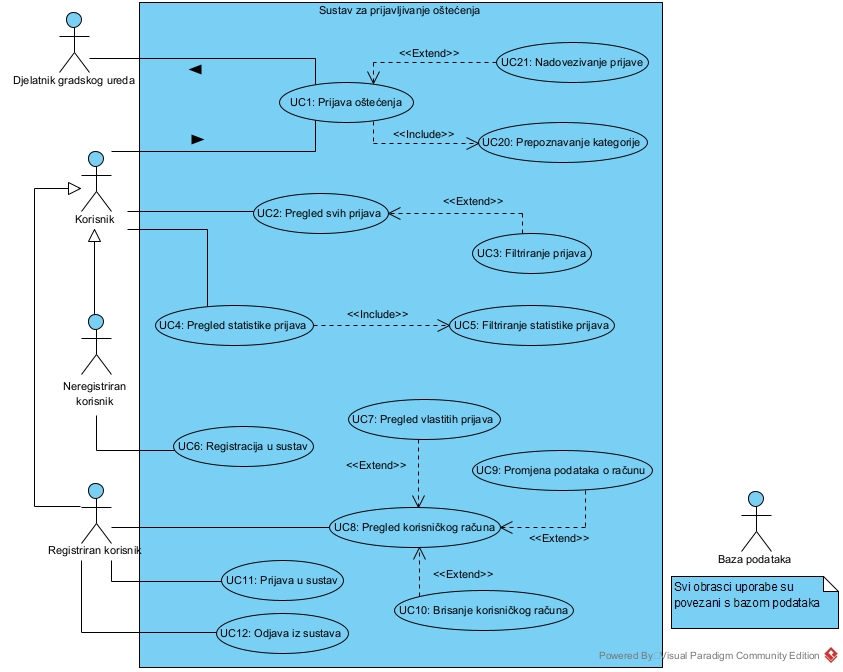
\includegraphics[width=\textwidth]{slike/Funkcionalnosti_korisnikaUCD.jpg} %veličina u odnosu na širinu linije
						\caption{Dijagram obrasca uporabe, funkcionalnosti korisnika}
						\label{fig:dijagramObrascaUporabe1} %label mora biti drugaciji za svaku sliku
					\end{figure}
					
					\begin{figure}[H]
						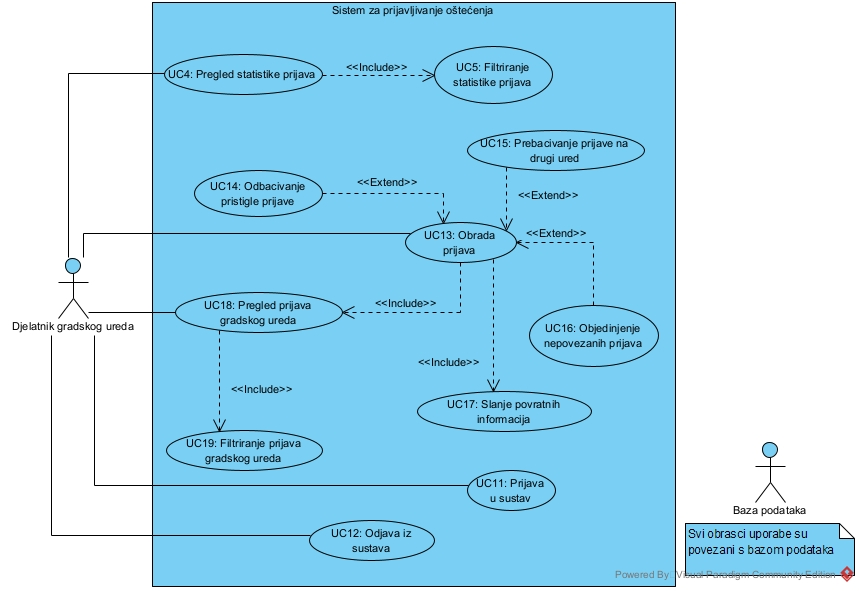
\includegraphics[width=\textwidth]{slike/Obrada_prijavaUCD.jpg} %veličina u odnosu na širinu linije
						\caption{Dijagram obrasca uporabe, obrada prijava}
						\label{fig:dijagramObrascaUporabe2} %label mora biti drugaciji za svaku sliku
					\end{figure}
					
				\eject		
				
			\subsection{Sekvencijski dijagrami}
				
				\textbf{\textit{dio 1. revizije}}\\
				
				\textbf{Obrasci uporabe - UC06, UC11 - Registracija u sustav, Prijava u sustav}
				
				Korisnik(može biti i djelatnik) na naslovnoj stranici odabire opciju prijave ili registracije te mu se zatim otvara prikladna stranica. Ako se radi o stranici za prijavu, korisnik unosi svoj email i zaporku i potvrđuje unos. Ako su uneseni podaci validni korisniku se prikazuje naslovna stranica za prijavljenog korisnika, odnosno za djelatnika gradskog ureda. U suprotnom se korisnika obavještava o grešci i ponovno traži unos podataka za prijavu. Ako se radi o stranici za registraciju, korisnik mora unijeti svoje ime, prezime, datum rođenja, email adresu i lozinku. Ako se registrira novi gradski ured, potrebno je označiti tu opciju. U tom slučaju se traži unos imena ureda, email adresa i lozinka. Sustav provjerava u bazi ako za danu email adresu već postoji korisnički račun. Ako račun već postoji, sustav korisniku javlja grešku i ponovno traži unos podataka za registraciju. Ako je unos dobar, korisniku se prikazuje naslovna stranica za prijavljenog korisnika, odnosno za djelatnika gradskog ureda. Korisnik ne mora odabrati opciju prijave ili registracije. U tom slučaju koristi stranicu kao anoniman neregistrirani korisnik. Djelatnik se mora prijaviti ili registrirati ured da bi obavljao svoju funkcionalnost.
				
				\begin{figure}[H]
					\includegraphics[width=\textwidth]{slike/Prijava_registracijaSD.jpg} %veličina u odnosu na širinu linije
					\caption{Sekvencijski dijagram, prijava/registracija}
					\label{fig:sekvencijskiDijagram1} %label mora biti drugaciji za svaku sliku
				\end{figure}
				\eject
				
				\textbf{Obrasci uporabe - UC1, UC2, UC3, UC4, UC5 - Prijava oštećenja, Pregled svih prijava, Filtriranje prijava, Pregled statistike prijava, Filtriranje statistike prijava}
				
				Korisnik odabire opciju podnošenja nove prijave oštećenja. U prijavi korisnik upisuje kratak naslov, opis oštećenja, lokaciju i kategoriju. Korisnik također može priložiti sliku oštećenja. Lokaciju korisnik može priložiti preko interaktivne karte, upisom adrese ili se lokacija može izvući iz metapodataka slike. Aplikacija će sama pokušati prepoznati kategoriju oštećenja i na temelju toga i ponuditi nadležan ured. Nakon podnošenja prijave korisnik dobiva kod prijave preko koje može pratiti njezino stanje. 
				Korisnik odabirom pregleda prijava može pregledavati postojeće aktive prijave u sustavu preko interaktivne karte. Prijave može dodatno filtrirati po vremenu, gradskom uredu i kategoriji. Odabirom neke prijave na karti korisniku se prikazuju podaci o toj prijavi.
				Korisnik odabirom statistike prijava također može pregledavati statistiku za prijave filtrirane po lokaciji, vremenu i gradskom uredu. U statistici se nalaze podaci o broju prijava svakog statusa, prosječno vrijeme koje je prijava imala neki status, prosječan broj prijava u danu i ukupan broj prijava.
				
				\begin{figure}[H]
					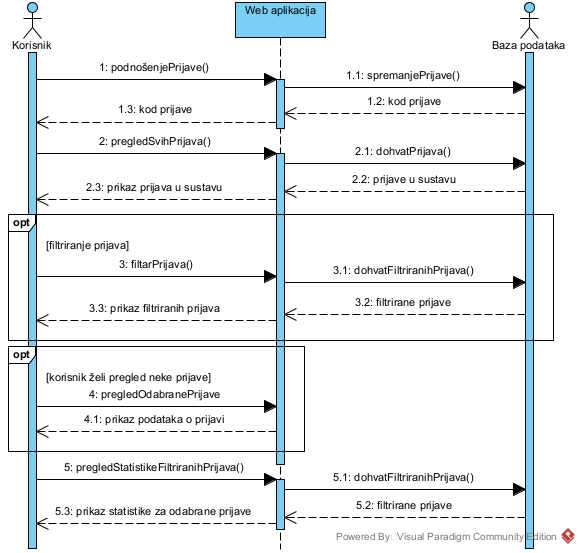
\includegraphics[width=\textwidth]{slike/Funkcionalnosti_korisnikaSD.jpg} %veličina u odnosu na širinu linije
					\caption{Sekvencijski dijagram, funkcionalnosti korisnika}
					\label{fig:sekvencijskiDijagram2} %label mora biti drugaciji za svaku sliku
				\end{figure}
				\eject
				
				\textbf{Obrasci uporabe - UC13, UC14, UC15, UC16, UC17, UC18, UC19 - Obrada prijava, Odbacivanje pristigle prijave, Prebacivanje prijave na drugi ured, Objedinjenje nepovezanih prijava, Slanje povratnih informacija, Pregled prijava gradskog ureda, filtriranje prijava gradskog ureda}
				
				Djelatnik gradskog ureda odabire jednu od 3 lista prijava, jedna za svaki status. Djelatnik može dodatno filtrirati prijave u listi po vremenu i kategoriji. Odabirom jedne od prijava djelatniku se prikazuju podaci o toj prijavi. Djelatnik dalje može promijeniti status prijave. Ako vidi da je oštećenje u toj prijavu već prijavljeno, djelatnik može odabrati sve takve prijave i objediniti ih. Ako utvrdi da njegov ured nije nadležan za ovu prijavu, djelatnik odabire nadležan ured i prosljeđuje mu prijavu. Ako je prijava u potpunosti nevaljana djelatnik ju može odbaciti. Bilo koja od ovih radnji nad prijavom rezultirati će slanjem povratne informacije korisniku koji je podnio prijavu, ako je taj korisnik registriran.
				
				\begin{figure}[H]
					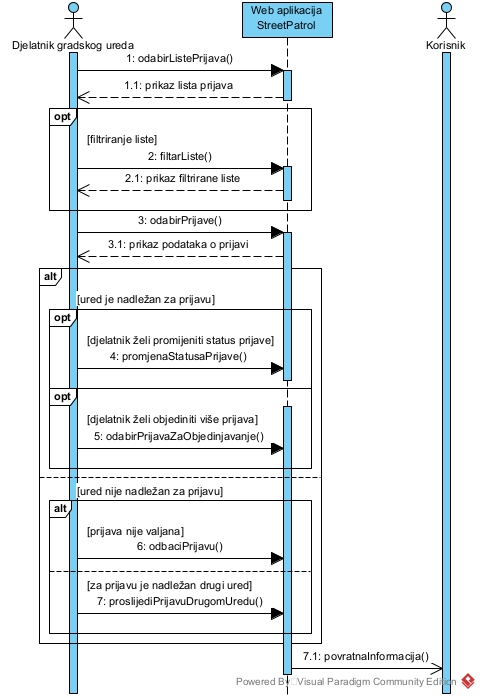
\includegraphics[width=\textwidth]{slike/Obrada_prijavaSD.jpg} %veličina u odnosu na širinu linije
					\caption{Sekvencijski dijagram, obrada prijava}
					\label{fig:sekvencijskiDijagram3} %label mora biti drugaciji za svaku sliku
				\end{figure}
				\eject


	
		\section{Ostali zahtjevi}
		
			\textbf{\textit{dio 1. revizije}}\\
			
			\begin{packed_item}
				\item Sustav treba podržati rad više korisnika u stvarnom vremenu
				\item Aplikacija podržava korisničko sučelje na hrvatskom i engleskom jeziku
				\item Sustav treba biti implementiran kao web aplikacija sa responzivnim dizajnom
				\item Rad i veza s bazom podataka moraju biti sigurni i pouzdani
				\item Aplikacija mora koristiti HTTPS protokol
				\item Aplikacija mora biti jednostavna za korištenje
				\item Neispravno korištenje korisničkog sučelja ne smije narušiti cijeloukupan rad sustava
				\item Izvršavanje bilo koje akcije na aplikaciji ne smije trajati dulje od 5 sekundi
				\item Osjetljivi podaci, kao što su lozinke korisnika, se u bazi moraju spremati u kriptiranom obliku
			\end{packed_item}
			